% Options for packages loaded elsewhere
\PassOptionsToPackage{unicode}{hyperref}
\PassOptionsToPackage{hyphens}{url}
%
\documentclass[
]{book}
\usepackage{lmodern}
\usepackage{amsmath}
\usepackage{ifxetex,ifluatex}
\ifnum 0\ifxetex 1\fi\ifluatex 1\fi=0 % if pdftex
  \usepackage[T1]{fontenc}
  \usepackage[utf8]{inputenc}
  \usepackage{textcomp} % provide euro and other symbols
  \usepackage{amssymb}
\else % if luatex or xetex
  \usepackage{unicode-math}
  \defaultfontfeatures{Scale=MatchLowercase}
  \defaultfontfeatures[\rmfamily]{Ligatures=TeX,Scale=1}
\fi
% Use upquote if available, for straight quotes in verbatim environments
\IfFileExists{upquote.sty}{\usepackage{upquote}}{}
\IfFileExists{microtype.sty}{% use microtype if available
  \usepackage[]{microtype}
  \UseMicrotypeSet[protrusion]{basicmath} % disable protrusion for tt fonts
}{}
\makeatletter
\@ifundefined{KOMAClassName}{% if non-KOMA class
  \IfFileExists{parskip.sty}{%
    \usepackage{parskip}
  }{% else
    \setlength{\parindent}{0pt}
    \setlength{\parskip}{6pt plus 2pt minus 1pt}}
}{% if KOMA class
  \KOMAoptions{parskip=half}}
\makeatother
\usepackage{xcolor}
\IfFileExists{xurl.sty}{\usepackage{xurl}}{} % add URL line breaks if available
\IfFileExists{bookmark.sty}{\usepackage{bookmark}}{\usepackage{hyperref}}
\hypersetup{
  pdftitle={일원배치법과 선형모형},
  pdfauthor={서울시립대 통계학과},
  hidelinks,
  pdfcreator={LaTeX via pandoc}}
\urlstyle{same} % disable monospaced font for URLs
\usepackage{color}
\usepackage{fancyvrb}
\newcommand{\VerbBar}{|}
\newcommand{\VERB}{\Verb[commandchars=\\\{\}]}
\DefineVerbatimEnvironment{Highlighting}{Verbatim}{commandchars=\\\{\}}
% Add ',fontsize=\small' for more characters per line
\usepackage{framed}
\definecolor{shadecolor}{RGB}{248,248,248}
\newenvironment{Shaded}{\begin{snugshade}}{\end{snugshade}}
\newcommand{\AlertTok}[1]{\textcolor[rgb]{0.94,0.16,0.16}{#1}}
\newcommand{\AnnotationTok}[1]{\textcolor[rgb]{0.56,0.35,0.01}{\textbf{\textit{#1}}}}
\newcommand{\AttributeTok}[1]{\textcolor[rgb]{0.77,0.63,0.00}{#1}}
\newcommand{\BaseNTok}[1]{\textcolor[rgb]{0.00,0.00,0.81}{#1}}
\newcommand{\BuiltInTok}[1]{#1}
\newcommand{\CharTok}[1]{\textcolor[rgb]{0.31,0.60,0.02}{#1}}
\newcommand{\CommentTok}[1]{\textcolor[rgb]{0.56,0.35,0.01}{\textit{#1}}}
\newcommand{\CommentVarTok}[1]{\textcolor[rgb]{0.56,0.35,0.01}{\textbf{\textit{#1}}}}
\newcommand{\ConstantTok}[1]{\textcolor[rgb]{0.00,0.00,0.00}{#1}}
\newcommand{\ControlFlowTok}[1]{\textcolor[rgb]{0.13,0.29,0.53}{\textbf{#1}}}
\newcommand{\DataTypeTok}[1]{\textcolor[rgb]{0.13,0.29,0.53}{#1}}
\newcommand{\DecValTok}[1]{\textcolor[rgb]{0.00,0.00,0.81}{#1}}
\newcommand{\DocumentationTok}[1]{\textcolor[rgb]{0.56,0.35,0.01}{\textbf{\textit{#1}}}}
\newcommand{\ErrorTok}[1]{\textcolor[rgb]{0.64,0.00,0.00}{\textbf{#1}}}
\newcommand{\ExtensionTok}[1]{#1}
\newcommand{\FloatTok}[1]{\textcolor[rgb]{0.00,0.00,0.81}{#1}}
\newcommand{\FunctionTok}[1]{\textcolor[rgb]{0.00,0.00,0.00}{#1}}
\newcommand{\ImportTok}[1]{#1}
\newcommand{\InformationTok}[1]{\textcolor[rgb]{0.56,0.35,0.01}{\textbf{\textit{#1}}}}
\newcommand{\KeywordTok}[1]{\textcolor[rgb]{0.13,0.29,0.53}{\textbf{#1}}}
\newcommand{\NormalTok}[1]{#1}
\newcommand{\OperatorTok}[1]{\textcolor[rgb]{0.81,0.36,0.00}{\textbf{#1}}}
\newcommand{\OtherTok}[1]{\textcolor[rgb]{0.56,0.35,0.01}{#1}}
\newcommand{\PreprocessorTok}[1]{\textcolor[rgb]{0.56,0.35,0.01}{\textit{#1}}}
\newcommand{\RegionMarkerTok}[1]{#1}
\newcommand{\SpecialCharTok}[1]{\textcolor[rgb]{0.00,0.00,0.00}{#1}}
\newcommand{\SpecialStringTok}[1]{\textcolor[rgb]{0.31,0.60,0.02}{#1}}
\newcommand{\StringTok}[1]{\textcolor[rgb]{0.31,0.60,0.02}{#1}}
\newcommand{\VariableTok}[1]{\textcolor[rgb]{0.00,0.00,0.00}{#1}}
\newcommand{\VerbatimStringTok}[1]{\textcolor[rgb]{0.31,0.60,0.02}{#1}}
\newcommand{\WarningTok}[1]{\textcolor[rgb]{0.56,0.35,0.01}{\textbf{\textit{#1}}}}
\usepackage{longtable,booktabs}
\usepackage{calc} % for calculating minipage widths
% Correct order of tables after \paragraph or \subparagraph
\usepackage{etoolbox}
\makeatletter
\patchcmd\longtable{\par}{\if@noskipsec\mbox{}\fi\par}{}{}
\makeatother
% Allow footnotes in longtable head/foot
\IfFileExists{footnotehyper.sty}{\usepackage{footnotehyper}}{\usepackage{footnote}}
\makesavenoteenv{longtable}
\usepackage{graphicx}
\makeatletter
\def\maxwidth{\ifdim\Gin@nat@width>\linewidth\linewidth\else\Gin@nat@width\fi}
\def\maxheight{\ifdim\Gin@nat@height>\textheight\textheight\else\Gin@nat@height\fi}
\makeatother
% Scale images if necessary, so that they will not overflow the page
% margins by default, and it is still possible to overwrite the defaults
% using explicit options in \includegraphics[width, height, ...]{}
\setkeys{Gin}{width=\maxwidth,height=\maxheight,keepaspectratio}
% Set default figure placement to htbp
\makeatletter
\def\fps@figure{htbp}
\makeatother
\setlength{\emergencystretch}{3em} % prevent overfull lines
\providecommand{\tightlist}{%
  \setlength{\itemsep}{0pt}\setlength{\parskip}{0pt}}
\setcounter{secnumdepth}{5}
\usepackage[onehalfspacing]{setspace}

\usepackage[hangul]{kotex}
\usepackage{fullpage}
\newcommand{\pardiff}[2]{\frac{\partial #1}{\partial #2 }}
\newcommand{\pardiffl}[2]{{\partial #1}/{\partial #2 }}
\newcommand{\pardiffd}[2]{\frac{\partial^2 #1}{\partial #2^t \partial #2 }}
\newcommand{\pardiffdd}[3]{\frac{\partial^2 #1}{\partial #2 \partial #3 }}

\newcommand{\bm}[1]{\boldsymbol{\mathbf{#1}}}

\usepackage{booktabs}
\usepackage{longtable}
\usepackage[bf,singlelinecheck=off]{caption}

%\setmainfont[UprightFeatures={SmallCapsFont=AlegreyaSC-Regular}]{Alegreya}

\usepackage{framed,color}
\definecolor{shadecolor}{RGB}{248,248,248}

\renewcommand{\textfraction}{0.05}
\renewcommand{\topfraction}{0.8}
\renewcommand{\bottomfraction}{0.8}
\renewcommand{\floatpagefraction}{0.75}

\renewenvironment{quote}{\begin{VF}}{\end{VF}}
\let\oldhref\href
\renewcommand{\href}[2]{#2\footnote{\url{#1}}}

\makeatletter
\newenvironment{kframe}{%
\medskip{}
\setlength{\fboxsep}{.8em}
 \def\at@end@of@kframe{}%
 \ifinner\ifhmode%
  \def\at@end@of@kframe{\end{minipage}}%
  \begin{minipage}{\columnwidth}%
 \fi\fi%
 \def\FrameCommand##1{\hskip\@totalleftmargin \hskip-\fboxsep
 \colorbox{shadecolor}{##1}\hskip-\fboxsep
     % There is no \\@totalrightmargin, so:
     \hskip-\linewidth \hskip-\@totalleftmargin \hskip\columnwidth}%
 \MakeFramed {\advance\hsize-\width
   \@totalleftmargin\z@ \linewidth\hsize
   \@setminipage}}%
 {\par\unskip\endMakeFramed%
 \at@end@of@kframe}
\makeatother

\makeatletter

\@ifundefined{Shaded}{
}{\renewenvironment{Shaded}{\begin{kframe}}{\end{kframe}}}
\makeatother

\newenvironment{rmdblock}[1]
  {
  \begin{itemize}
  \renewcommand{\labelitemi}{
    \raisebox{-.7\height}[0pt][0pt]{
      {\setkeys{Gin}{width=3em,keepaspectratio}\includegraphics{images/#1}}
    }
  }
  \setlength{\fboxsep}{1em}
  \begin{kframe}
  \item
  }
  {
  \end{kframe}
  \end{itemize}
  }
  
\newenvironment{rmdnote}
  {\begin{rmdblock}{note}}
  {\end{rmdblock}}
  
\newenvironment{rmdcaution}
  {\begin{rmdblock}{caution}}
  {\end{rmdblock}}
  
\newenvironment{rmdimportant}
  {\begin{rmdblock}{important}}
  {\end{rmdblock}}
  
\newenvironment{rmdtip}
  {\begin{rmdblock}{tip}}
  {\end{rmdblock}}
  
\newenvironment{rmdwarning}
  {\begin{rmdblock}{warning}}
  {\end{rmdblock}}
  


%\usepackage{makeidx}
%\makeindex

\urlstyle{tt}

\usepackage{amsthm}
\makeatletter
 \def\thm@space@setup{%
   \thm@preskip=8pt plus 2pt minus 4pt
   \thm@postskip=\thm@preskip
}
\makeatother

\frontmatter

\ifluatex
  \usepackage{selnolig}  % disable illegal ligatures
\fi
\usepackage[]{natbib}
\bibliographystyle{apalike}

\title{일원배치법과 선형모형}
\author{서울시립대 통계학과}
\date{2021-04-08}

\begin{document}
\maketitle

{
\setcounter{tocdepth}{1}
\tableofcontents
}
\hypertarget{uxc11cuxbb38}{%
\chapter*{서문}\label{uxc11cuxbb38}}


일원배치 실험계획법의 목적은 서로 다른 처리의 효과가 같은지 다른지 알아보는 것이다. 따라서 분삽분석표를 이용하여 다음과 같은 가설을 검정한다.

\[ H_0 : \alpha_1 = \alpha_2 = \cdots = \alpha_a \]

만약 위의 귀무가설을 기각하지 못했다면 처리의 효과들이 모두 같으므로 더 이상의 추론은 소용이 없다.
하지만 만약 귀무가설을 기각하게 되면 처리 효과들이 어떻게 다른지 추론해 보아야 한다.

교과서 3.5 절과 강의노트에서 각 처리에 대한 반응값 의 평균 \(\mu+\alpha_i\)과 각 처리간의 차이 \(\alpha_i - \alpha_j\)에 대한 신뢰구간과 가설 검정을 다루었다.

이 강의에서는 일원배치에서 처리 효과를 비교하는 통계적 방법들에 대하여 더욱 자세하게 알아보려고 한다.

\begin{rmdcaution}
교과서에서는 반응 변수를 \(x\) 로 표현하였는데 이 강의에서는 \(y\) 로 표시할 것이다.
\end{rmdcaution}

\begin{center}\rule{0.5\linewidth}{0.5pt}\end{center}

이 노트는 분산분석 후에 여러 개의 수준에 대한 비교를 할 때 통계적 방법에 대한 이론과 예제에 대한 강의자료입니다.
이 노트에 있는 R 프로그램을 실행하려면 다음과 같은 패키지들이 필요하다.

\begin{verbatim}
library(dplyr)
library(tidyr)
library(ggplot2)
library(agricolae)
library(emmeans)
\end{verbatim}

\mainmatter

\hypertarget{onewaylse}{%
\chapter{일원배치 모형과 최소제곱법}\label{onewaylse}}

\hypertarget{uxcd5cuxc18cuxc81cuxacf1uxbc95uxacfc-uxc81cuxc57duxc870uxac74}{%
\section{최소제곱법과 제약조건}\label{uxcd5cuxc18cuxc81cuxacf1uxbc95uxacfc-uxc81cuxc57duxc870uxac74}}

이제 일원배치법에 대한 통계적 모형에서 모수에 대한 추정을 생각해 보자.

\begin{equation}
y_{ij} = \mu + \alpha_i + e_{ij} 
\label{eq:oneway}
\end{equation}

추정해야할 모수는 전체 평균 \(\mu\)와 각 그룹의 처리 효과 \(\alpha_i\) 그리고 분산 \(\sigma_E^2\)이다. 전체 평균과 그룹의 효과는 오차제곱합(Sum of Square Error; SSE)을 최소로 하는 모수를 추정하는 최소제곱법(Least Square method; LS)으로 구할 수 있다.

\begin{equation} 
 \min_{\mu, \alpha_1, \dots \alpha_a} \sum_{i=1}^a \sum_{j=1}^r 
(y_{ij} - \mu -\alpha_i)^2 =\min_{\mu, \alpha_1, \dots \alpha_a} SSE 
\label{eq:lsesse}
\end{equation}

위의 오차제곱합이 모든 모수에 대하여 미분가능한 이차식으므로 최소제곱 추정량은 제곱합을 모수에 대하여 미분하고 0 으로 놓아 방정식을 풀어서 얻을 수 있다.

오차제곱합을 모수 \(\mu\)와 \(\alpha_1,\alpha_2,\dots,\alpha_a\) 로 미분하여 0 으로 놓은 방정식은 다음과 같다.

\begin{align*}
& \pardiff{}{\mu} SSE = -2 \sum_{i=1}^a \sum_{j=1}^r (y_{ij} - \mu -\alpha_i) = 0 \\
& \pardiff{}{\alpha_i} SSE = -2 \sum_{j=1}^r (y_{ij} - \mu -\alpha_i) = 0 , \quad i=1,2,\dots, a 
\end{align*}

위의 방정식을 정리하면 다음과 같은 \(a+1\)개의 방정식을 얻는다.

\begin{align}
   \mu +\frac{ \sum_{i=1}^a \alpha_i}{a} & = \bar {\bar y}\\
   \mu + \alpha_1  & =  \bar {y}_{1.} \\
   \mu + \alpha_2  & =  \bar {y}_{2.} \\
         \cdots & \cdots \\
   \mu + \alpha_a  & =  \bar {y}_{a.} \\
\label{eq:normaleq1}   
\end{align}

위의 방정식에서 첫 번째 방정식은 다른 \(a\)개의 방정식을 모두 합한 방정식과 같다. 따라서 모수는 \(a+1\)개이지만 실제 방정식의 개수는 \(a\)개이므로
유일한 해가 얻어지지 않는다. 따라서 유일한 해를 구하려면 하나의 제약조건이 필요하며 일반적으로 다음과 같은 두 개의 조건 중 하나를 사용한다.

\hypertarget{set-to-zero-condition}{%
\subsection{set-to-zero condition}\label{set-to-zero-condition}}

첫 번째 효과 \(\alpha_1\)를 0으로 놓는 조건을 주는 것이다 (\(\alpha_1=0\)). set-to-zero 조건 하에서는 다음과 같은 추정량이 얻어진다.

\begin{equation}
\hat \mu = \bar {y}_{1.}, \quad \hat \alpha_1=0, ~~  \hat \alpha_i = \bar {y}_{i.} -\bar {y}_{1.},~~i=2,\dots,a
\label{eq:setzeroest}
\end{equation}

\hypertarget{sum-to-zero-condition}{%
\subsection{sum-to-zero condition}\label{sum-to-zero-condition}}

처리들의 효과의 합은 0이라는 조건을 주는 것이다 ( \(\sum_{i=1}^a \alpha_i=0\)). sum-to-zero 조건에서는 계수의 추정치가 다음과 같이 주어진다.

\begin{equation}
\hat \mu = \bar {\bar {y}}, \quad \hat \alpha_i = \bar {y}_{i.} -\bar {\bar {y}},~~i=1,2,\dots,a 
\label{eq:sumzeroest}
\end{equation}

여기서 유의할 점은 \textbf{개별 모수들의 추정량은 조건에 따라서 달라지지만 집단의 평균을 나타내는 모수 \(\mu+ \alpha_i\) 에 대한 추정량은 언제나 같다}.

\[ \widehat{\mu+ \alpha_i} = \hat \mu + \hat {\alpha}_i =  \bar {y}_{i.} \]

만약에 자료를 아래와 같은 평균 모형으로 나타낼 경우에는 각 평균 \(\mu_i\) 는 각 그룹의 표본 평균으로 추정된다.

\[ y_{ij} = \mu_i + e_{ij} \]

평균 모형에서 각 그룹의 모평균에 대한 최소제곱 추정량은 \(\hat \mu_i = \bar {y}_{i.}\) 이며 이는 주효과 모형에서의 추정량과 동일하다.

또한 모형에 관계없이 오차항의 분산 \(\sigma_E^2\) 에 대한 추정량은 다음과 같이 주어진다.

\begin{equation*} 
\hat \sigma_E^2 = \frac{ \sum_i \sum_j (y_{ij} - \hat \mu -\hat \alpha_i )^2}{a(r-1)}
\end{equation*}

\hypertarget{uxc120uxd615uxbaa8uxd615uxacfc-uxc81cuxc57d-uxc870uxac74}{%
\section{선형모형과 제약 조건}\label{uxc120uxd615uxbaa8uxd615uxacfc-uxc81cuxc57d-uxc870uxac74}}

일원배치 모형 \eqref{eq:oneway}를 다음과 같은 벡터를 이용한 선형모형(linear model, regression model) 형태로 나타내고자 한다.

\begin{equation}
\bm y = \bm X \bm \beta +\bm e
\label{eq:lm}
\end{equation}

위의 선형모형식의 요소 \(\bm y\), \(\bm X\), \(\bm \beta\), \(\bm e\)는 다음과 같은 벡터와 행렬로 표현된다.

\begin{equation}
\begin{bmatrix}
y_{11} \\
y_{12} \\
\vdots \\
y_{1r} \\
y_{21} \\
y_{22} \\
\vdots \\
y_{2r} \\
\vdots \\
y_{a1} \\
y_{a2} \\
\vdots \\
y_{ar} \\
\end{bmatrix} 
 =
\begin{bmatrix}
1 & 1 & 0 & . & . & 0 \\
1 & 1 & 0 & . & . & 0 \\
1 & \vdots & \vdots & \vdots & \vdots & \vdots \\
1 & 1 & 0 & . & . & 0 \\
1 & 0 & 1 & . & . & 0 \\
1 & 0 & 1 & . & . & 0 \\
1 & \vdots & \vdots & \vdots & \vdots & \vdots \\
1 & 0 & 1 & . & . & 0 \\
\vdots & \vdots & \vdots & \vdots & \vdots & \vdots \\
1 & 0 & 0 & . & . & 1 \\
1 & 0 & 0 & . & . & 1 \\
1 & \vdots & \vdots & \vdots & \vdots & \vdots \\
1 & 0 & 0 & . & . & 1 \\
\end{bmatrix}
\begin{bmatrix}
\mu \\
\alpha_{1} \\
\alpha_{2} \\
\vdots \\
\alpha_{a} \\
\end{bmatrix} +
\begin{bmatrix}
e_{11} \\
e_{12} \\
\vdots \\
e_{1r} \\
e_{21} \\
e_{22} \\
\vdots \\
e_{2r} \\
\vdots \\
e_{a1} \\
e_{a2} \\
\vdots \\
e_{ar} \\
\end{bmatrix}
\label{eq:lm2}
\end{equation}

이제 위에서 논의한 최소제곱법을 선형 모형 \eqref{eq:lm} 에 적용하면 다음과 같이 표현할 수 있다.

\begin{equation} 
 \min_{\mu, \alpha_1, \dots \alpha_a} \sum_{i=1}^a \sum_{j=1}^r 
(y_{ij} - \mu -\alpha_i)^2 = \min_{\bm \beta } ( \bm y -  \bm X \bm \beta )^t( \bm y -  \bm X \bm \beta ) 
 \label{eq:rsq2}
 \end{equation}

최소제곱법의 기준을 만족하는 계수 \(\bm \beta\)는 다음과 같은 정규방정식(normal equation)의 해(solution)이다.

\begin{equation}
\bm X^t \bm X \bm \beta = \bm X^t \bm y
\label{eq:normaleq2}
\end{equation}

정규방정식 \eqref{eq:normaleq2} 을 일워배치의 선형모형식 \eqref{eq:lm2} 에 나타난 \(\bm y\), \(\bm X\)로 이용하여 나타내면 다음과 같다.

\begin{equation}
\begin{bmatrix}
ar   & r & r & \cdot & \cdot & r \\
r & r &  0  & \cdot & \cdot & 0 \\
r & 0   & r  & \cdot & \cdot & 0 \\
\cdot & \cdot   & \cdot  & \cdot & \cdot & \cdot \\
\cdot & \cdot   & \cdot  & \cdot & \cdot & \cdot \\
r & 0   &  0   & \cdot & \cdot & r \\
\end{bmatrix}
\begin{bmatrix}
\mu \\
\alpha_{1} \\
\alpha_{2} \\
\cdot \\
\cdot \\
\alpha_{a} \\
\end{bmatrix}
=
\begin{bmatrix}
ar \bar {\bar y} \\
r {\bar y}_{1.}\\
r \bar y_{2.}\\
\cdot \\
\cdot \\
r \bar y_{a.}
\end{bmatrix}
\label{eq:normaleq3}
\end{equation}

정규방정식 \eqref{eq:normaleq3} 는 위에서 구한 최소제곱법에서 유도된 방정식 \eqref{eq:normaleq1} 과 같다.

여기서 유의할 점은 선형모형식 \eqref{eq:lm2} 의 계획행렬 \(\bm X\) 가 완전 계수(full rank) 행렬이 아니다.
계획행렬 \(\bm X\)의 첫 번째 열은 다른 열을 합한 것과 같다.
또한 정규 방정식 \eqref{eq:normaleq3}에서 \(\bm X^t \bm X\) 행렬도 완전계수 행렬이 아니다.
따라서 \(\bm X^t \bm X\) 행렬의 역행렬은 존재하지 않는다.

이러한 이유로 모수에 대한 유일한 추정량이 존재하지 않기 때문에 앞에서 언급한 제약 조건을 고려해야 정규방정식을 풀 수 있다.

\hypertarget{set-to-zero-uxc870uxac74uxc5d0uxc11cuxc758-uxbaa8uxd615uxacfc-uxcd5cuxc18cuxc81cuxacf1-uxcd94uxc815uxb7c9}{%
\subsection{Set-to-zero 조건에서의 모형과 최소제곱 추정량}\label{set-to-zero-uxc870uxac74uxc5d0uxc11cuxc758-uxbaa8uxd615uxacfc-uxcd5cuxc18cuxc81cuxacf1-uxcd94uxc815uxb7c9}}

만약 Set-to-zero 조건을 가정한다면 모수에서 \(\alpha_1\)을 제외하고 선형모형식 \eqref{eq:lm2}를 다음과 같이 다시 표현할 수 있다.\\
효과 \(\alpha_1\)을 0 으로 놓는다는 것은 \(\alpha_1\)을 추정할 필요가 없으므로 모수벡터 \(\bm \beta\) 에서 \(\alpha_1\)를 빼고
게획행렬에서도 대응하는 열을 제거하는 것이다.

\begin{equation}
\begin{bmatrix}
y_{11} \\
y_{12} \\
\vdots \\
y_{1r} \\
y_{21} \\
y_{22} \\
\vdots \\
y_{2r} \\
\vdots \\
y_{a1} \\
y_{a2} \\
\vdots \\
y_{ar} \\
\end{bmatrix} 
 =
\begin{bmatrix}
1 &  0 & . & . & 0 \\
1 &  0 & . & . & 0 \\
1 &  \vdots & \vdots & \vdots & \vdots \\
1 &  0 & . & . & 0 \\
1 &  1 & . & . & 0 \\
1 &  1 & . & . & 0 \\
1 &  \vdots & \vdots & \vdots & \vdots \\
1 &  1 & . & . & 0 \\
\vdots &  \vdots & \vdots & \vdots & \vdots \\
1 &  0 & . & . & 1 \\
1 &  0 & . & . & 1 \\
1 &  \vdots & \vdots & \vdots & \vdots \\
1 &  0 & . & . & 1 \\
\end{bmatrix}
\begin{bmatrix}
\mu \\
\alpha_{2} \\
\alpha_{3} \\
\vdots \\
\alpha_{a} \\
\end{bmatrix} +
\begin{bmatrix}
e_{11} \\
e_{12} \\
\vdots \\
e_{1r} \\
e_{21} \\
e_{22} \\
\vdots \\
e_{2r} \\
\vdots \\
e_{a1} \\
e_{a2} \\
\vdots \\
e_{ar} \\
\end{bmatrix}
\label{eq:lm-zero}
\end{equation}

이제 수정된 모형식 \eqref{eq:lm-zero} 에 최소제곱법을 적용하여 정규방정식을 구하면 다음과 같은 방정식을 얻는다.

\begin{equation}
\begin{bmatrix}
ar   & r & r & \cdot & \cdot & r \\
r & r &  0  & \cdot & \cdot & 0 \\
r & 0   & r  & \cdot & \cdot & 0 \\
\cdot & \cdot   & \cdot  & \cdot & \cdot & \cdot \\
\cdot & \cdot   & \cdot  & \cdot & \cdot & \cdot \\
r & 0   &  0   & \cdot & \cdot & r \\
\end{bmatrix}
\begin{bmatrix}
\mu \\
\alpha_{2} \\
\alpha_{3} \\
\cdot \\
\cdot \\
\alpha_{a} \\
\end{bmatrix}
=
\begin{bmatrix}
ar \bar {\bar y} \\
r {\bar y}_{2.}\\
r \bar y_{3.}\\
\cdot \\
\cdot \\
r \bar y_{a.}
\end{bmatrix}
\label{eq:normaleq-zero}
\end{equation}

위의 정규방정 \eqref{eq:normaleq-zero} 를 풀면 위에서 언급한 sum-to-zero 조건에서 구해지는 모수의 추정량 \eqref{eq:setzeroest}를 얻을 수 있다.

\hypertarget{sum-to-zero-uxc870uxac74uxc5d0uxc11cuxc758-uxbaa8uxd615uxacfc-uxcd5cuxc18cuxc81cuxacf1-uxcd94uxc815uxb7c9}{%
\subsection{Sum-to-zero 조건에서의 모형과 최소제곱 추정량}\label{sum-to-zero-uxc870uxac74uxc5d0uxc11cuxc758-uxbaa8uxd615uxacfc-uxcd5cuxc18cuxc81cuxacf1-uxcd94uxc815uxb7c9}}

이제 Sum-to-zero 조건에서 모수의 추정에 대해 알아보자. 조건 \(\sum_{i=1}^a \alpha_i =0\) 조건을 마지막 모수 \(\alpha_a\)에 대하여 표현하면 다음과 같다.

\[ \alpha_a = -\alpha_1 - \alpha_2 - \dots - \alpha_{a-1} \]

따라서 마지막 처리 \(\alpha_a\) 에 대한 관측값에 대한 모형은 다음과 같아 쓸 수 있다.

\[ y_{aj} = \mu + \alpha_a + e_{aj} = \mu +( -\alpha_1 - \alpha_2 - \dots - \alpha_{a-1}) + e_{ij} \]

이러한 결과를 모형방정식에 반영한다. 즉, 모수벡터 \(\bm \beta\) 에서 \(\alpha_a\)를 제거하고 게획행렬에 위의 마지막 처리에 대한 효과식을 반영하면 다음과 같은 선형모형식을 얻는다.

\begin{equation}
\begin{bmatrix}
y_{11} \\
y_{12} \\
\vdots \\
y_{1r} \\
y_{21} \\
y_{22} \\
\vdots \\
y_{2r} \\
\vdots \\
y_{a1} \\
y_{a2} \\
\vdots \\
y_{ar} \\
\end{bmatrix} 
 =
\begin{bmatrix}
1 & 1 & 0 & . & . & 0 \\
1 & 1 & 0 & . & . & 0 \\
1 & \vdots & \vdots & \vdots & \vdots & \vdots \\
1 & 1 & 0 & . & . & 0 \\
1 & 0 & 1 & . & . & 0 \\
1 & 0 & 1 & . & . & 0 \\
1 & \vdots & \vdots & \vdots & \vdots & \vdots \\
1 & 0 & 1 & . & . & 0 \\
\vdots & \vdots & \vdots & \vdots & \vdots & \vdots \\
1 & 0 & 0 & . & . & 1 \\
1 & 0 & 0 & . & . & 1 \\
1 & \vdots & \vdots & \vdots & \vdots & \vdots \\
1 & 0 & 0 & . & . & 1 \\
1 & 0 & 0 & . & . & 1 \\
1 & -1 & -1 & . & . & -1 \\
1 & -1 & -1 & . & . & -1 \\
1 & \vdots & \vdots & \vdots & \vdots & \vdots \\
1 & -1 & -1 & . & . & -1 \\
1 & -1 & -1 & . & . & -1 \\
\end{bmatrix}
\begin{bmatrix}
\mu \\
\alpha_{1} \\
\alpha_{2} \\
\vdots \\
\alpha_{a-1} \\
\end{bmatrix} +
\begin{bmatrix}
e_{11} \\
e_{12} \\
\vdots \\
e_{1r} \\
e_{21} \\
e_{22} \\
\vdots \\
e_{2r} \\
\vdots \\
e_{a1} \\
e_{a2} \\
\vdots \\
e_{ar} \\
\end{bmatrix}
\label{eq:lm-sum}
\end{equation}

이제 수정된 모형식 \eqref{eq:lm-sum} 에 최소제곱법을 적용하여 정규방정식을 구하면 다음과 같은 방정식을 얻는다.

\begin{equation}
\begin{bmatrix}
ar   & 0 & 0 & \cdot & \cdot & 0 \\
0 & 2r &  r  & \cdot & \cdot & r \\
0 & r   & 2r  & \cdot & \cdot & r \\
\cdot & \cdot   & \cdot  & \cdot & \cdot & \cdot \\
\cdot & \cdot   & \cdot  & \cdot & \cdot & \cdot \\
0 & r   &  r   & \cdot & \cdot & 2r \\
\end{bmatrix}
\begin{bmatrix}
\mu \\
\alpha_{2} \\
\alpha_{3} \\
\cdot \\
\cdot \\
\alpha_{a-1} \\
\end{bmatrix}
=
\begin{bmatrix}
ar \bar {\bar y} \\
r {\bar y}_{2.}-r {\bar y}_{a.} \\
r \bar y_{3.}-r {\bar y}_{a.}\\
\cdot \\
\cdot \\
r \bar y_{a-1,.} -r {\bar y}_{a.}
\end{bmatrix}
\label{eq:normaleq-sum}
\end{equation}

위의 정규방정 \eqref{eq:normaleq-sum} 를 풀면 위에서 언급한 sum-to-zero 조건에서 구해지는 모수의 추정량 \eqref{eq:sumzeroest}를 얻을 수 있다.

\hypertarget{estimable}{%
\chapter{추정 가능한 함수}\label{estimable}}

\hypertarget{uxc77cuxc6d0uxbc30uxce58uxbc95uxc5d0-uxcd94uxc815uxac00uxb2a5uxd55c-uxbaa8uxc218}{%
\section{일원배치법에 추정가능한 모수}\label{uxc77cuxc6d0uxbc30uxce58uxbc95uxc5d0-uxcd94uxc815uxac00uxb2a5uxd55c-uxbaa8uxc218}}

앞 절에서 보았듯이 일원배치법을 선형 모형식으로 표현하는 경우 평균에 대한 모수는 모두 \(a+1\) 개가 있다.

\[ \mu, \alpha_1, \alpha_2, \cdots, \alpha_a \]

하지만 모형식에서 계획행렬 \(\bm X\)가 완전 계수 행렬이 아니기 때문에 1개의 제약 조건을 가정하고 모수를 추정하였다.
하지만 제약 조건이 달라지면 각 모수의 추정량이 달라지기 때문에 각 모수는 유일한 값으로 추정이 불가능하다.

이렇게 각 모수들은 제약 조건에 따라서 유일하게 추정이 불가능하지만 앞 절에서 보았듯이 \(\mu + \alpha_i\) 에 대한 추정량은 제약조건에 관계없이
표본 평균 \(\bar y_{i.}\)으로 동일하게 추정되어 진다.

그러면 어떤 모수들은 유일하게 추정이 불가능하고 어떤 모수들이 유일하게 추정이 가능할까?

이제 제약조건이 달라도 유일하게 추정이 가능한 모수들의 형태를 살펴보자.

\hypertarget{uxcd94uxc815uxac00uxb2a5uxd55c-uxbaa8uxc218uxc758-uxd568uxc218}{%
\section{추정가능한 모수의 함수}\label{uxcd94uxc815uxac00uxb2a5uxd55c-uxbaa8uxc218uxc758-uxd568uxc218}}

선형모형 \(\bm y =\bm X \bm \beta + \bm e\) 에서 계획행렬 \(\bm X\)의 계수가 완전하지 않으면 모수 벡터 \(\bm \beta\)는 유일한 값으로 추정할 수 없다.

이제 임의의 벡터 \(\bm c\)가 있을 때 모수들의 선형결합 \(\psi = \bm c^t \bm \beta\)를 고려하자.

예를 들어 일원배치 모형에서는 다음과 같은 모수들의 선형결합을 고려하는 것이다.

\[ \psi = \bm c^t \bm \beta = 
[ c_0~ c_1~ c_2~ \cdots~~c_a] 
\begin{bmatrix}
\mu \\
\alpha_1 \\
\alpha_2 \\
\vdots \\
\alpha_a
\end{bmatrix}
=c_0 \mu + c_1 \alpha_1 + c_2 \alpha_2 + \cdots + c_a \alpha_a \]

위에서 본 것처럼 하나의 모수 \(\alpha_1\)에 대한 유일한 추정은 불가능하다.

\[  \alpha_1 = (0) \mu + (1) \alpha_1 + (0) \alpha_2 + \cdots + (0) \alpha_a \]

하지만 모수의 조합 \(\mu+ \alpha_2\) 은 유일한 추정이 가능하다.

\[  \mu + \alpha_1 = (1) \mu + (1) \alpha_1 + (0) \alpha_2 + \cdots + (0) \alpha_a \]

이제 문제는 선형조합 \(\psi= \bm c^t \bm \beta\) 에서 계수들 \(c_0, c_1, \dots, c_a\)가 어떤 값을 가지는 경우 유일한 추정이 가능한 지 알아내는 것이다.

이제 \(\psi = \bm c^t \bm \beta\) 에 대한 유일한 추정량 \(\hat \psi\) 이 있다고 가정하자. 선형 모형에서 추정량 \(\hat \psi\)의 형태는 관측값에 대한 선형함수가 되어야 한다. 따라서 추정량을 \(\hat \psi = \bm a^t \bm y\) 로 나타낼 수 있다. 이제 추정량 \(\hat \psi\)의 기대값은 \(\psi=\bm c^t \bm \beta\)이어야 하므로 다음이 성립해야 한다.

\[ E(\hat \psi| \bm X) = E(\bm a^t \bm y| \bm X) = \bm a^t E(\bm y| \bm X) = \bm a^t \bm X \bm \beta = \bm c^t \bm \beta \]

위의 식에서 가장 마지막 두 항의 관계를 보면 다음이 성립해야 한다.

\begin{equation}
\bm a^t \bm X = \bm c^t  \quad \text{ equivalently }\quad \bm c = \bm X^t \bm a
\label{eq:estimable}
\end{equation}

즉 추정가능한 모수의 조합 \(\psi = \bm c^t \bm \beta\)에서 \textbf{계수 벡터 \(\bm c\) 는 계획행렬에 있는 행들의 선형 조합}으로 표시되어야 한다는 것이다. 이렇게 유일하게 추정이 가능한
모수의 조합을 \textbf{추정가능한 함수(estimable function)}이라고 한다.

\hypertarget{uxc608uxc81c}{%
\section{예제}\label{uxc608uxc81c}}

2개의 수준이 있고 반복이 2번 있는 일원배치 \((a=2,r=2)\) 에 대한 선형모형 \eqref{eq:lm2}을 생각해보자. 이 경우 계획행렬 \(\bm X\) 과 모수벡터 \(\bm \beta\) 는 다음과 같다.

\begin{equation}
\bm X = 
\begin{bmatrix}
1 & 1 & 0  \\
1 & 1 & 0  \\
1 & 0 & 1  \\
1 & 0 & 1  
\end{bmatrix}
\quad 
\bm \beta = 
\begin{bmatrix}
\mu \\
\alpha_1 \\
\alpha_2 
\end{bmatrix}
\end{equation}

이제 유일하게 추정 가능한 모수 조합 \(\psi\) 은 어떤 형태일까?

\[ \psi = \bm c^t \bm \beta = c_0 \mu + c_1 \alpha_1 + c_2 \alpha_2 \]

위의 식 \eqref{eq:estimable}에서 추정가능한 모수의 조합에 대한 계수 벡터 \(\bm c\)
는 다음과 같은 조건을 만족해야 한다.

\[ \bm c = {\bm X}^t \bm a \]

이제 임의의 벡터 \(\bm a\) 에 대하여 \(\bm c= \bm X^t \bm a\)의 형태를 보자.

\begin{align}
\bm c &= 
\bm X^t \bm a \\ & = 
\begin{bmatrix}
1 & 1 & 1 & 1  \\
1 & 1 & 0 & 0  \\
0 & 0 & 1 & 1  
\end{bmatrix}
\begin{bmatrix}
a_1 \\
a_2 \\
a_3 \\
a_4 
\end{bmatrix} \\
& = 
a_1 
\begin{bmatrix}
1 \\
1 \\
0 
\end{bmatrix}
+
a_2
\begin{bmatrix}
1 \\
1 \\
0 
\end{bmatrix}
+ 
a_3 
\begin{bmatrix}
1 \\
0 \\
1 
\end{bmatrix}
+
 a_4
\begin{bmatrix}
1 \\
0 \\
1 
\end{bmatrix} \\
& = 
(a_1 + a_2)
\begin{bmatrix}
1 \\
1 \\
0 
\end{bmatrix}
+ 
(a_3 + a_4)
\begin{bmatrix}
1 \\
0 \\
1 
\end{bmatrix} \\
&= 
b_1
\begin{bmatrix}
1 \\
1 \\
0 
\end{bmatrix}
+ 
b_2
\begin{bmatrix}
1 \\
0 \\
1 
\end{bmatrix} 
\label{eq:esticond}
\end{align}

이제 \textbf{\(\bm X^t \bm a\) 는 계획행렬 \(\bm X\)에 있는 유일한 행들의 선형조합}임을 알 수 있다.

\begin{rmdnote}
위의 식 \eqref{eq:esticond} 에서 유의할 점은 벡터 \(\bm a=[a_1 ~a_2~a_3~a_4]^t\)는 임의로 주어진 벡터이다.

식 \eqref{eq:esticond} 에서 \(a_1=1\), \(a_2=1\) 인 경우는 \(a_1=2\), \(a_2=0\) 인 경우와 동일하다.
\end{rmdnote}

따라서 유일하게 추정 가능한 모수의 선형조합 \(\psi = \bm c^t \bm \beta\) 에 대한 계수 벡터 \(\bm c =[ c_0 ~ c_1 ~ c_2]^t\) 는 계획행렬 \(\bm X\)의 유일한 행들의 선형 조합으로 구성되어야 한다.

\begin{equation}
\bm c =
\begin{bmatrix}
c_0 \\
c_1 \\
c_2 
\end{bmatrix}
= 
b_1
\begin{bmatrix}
1 \\
1 \\
0 
\end{bmatrix}
+ 
b_2
\begin{bmatrix}
1 \\
0 \\
1 
\end{bmatrix}
\label{eq:esticond2}
\end{equation}

\begin{itemize}
\tightlist
\item
  처리의 효과를 나타내는 모수 \(\alpha_i\)는 추정이 불가능하다.
\end{itemize}

첫 번째 처리에 대한 효과 모수 \(\alpha_1\) 를 선형조합으로 나타내면

\[ \alpha_1 = c_0 \mu + c_1 \alpha_1 + c_2 \alpha_2 = (0) \mu + (1) \alpha_1 + (0) \alpha_2 \]

따라서 조건 \eqref{eq:esticond2} 에서 \(\bm c^t = [0~1~0]\)을 만들수 있는 계수 \(b_1\)과 \(b_2\)를 찾아야 하는데 이는 불가능하다. 따라서 모수 \(\alpha_1\) 은 추정 불가능하다.

\begin{equation*}
\bm c =
\begin{bmatrix}
0 \\
1 \\
0 
\end{bmatrix}
= 
b_1
\begin{bmatrix}
1 \\
1 \\
0 
\end{bmatrix}
+ 
b_2
\begin{bmatrix}
1 \\
0 \\
1 
\end{bmatrix}
\end{equation*}

\begin{itemize}
\tightlist
\item
  처리의 평균을 나타내는 모수의 조합 \(\mu + \alpha_i\)는 추정이 가능하다.
\end{itemize}

모수 조합 \(\mu + \alpha_1\) 를 선형조합으로 나타내면

\[ \mu + \alpha_1 = c_0 \mu + c_1 \alpha_1 + c_2 \alpha_2 = (1) \mu + (1) \alpha_1 + (0) \alpha_2 \]

따라서 조건 \eqref{eq:esticond2} 에서 \(\bm c^t = [1~1~0]\)을 만들수 있는 계수는 \(b_1=1\)과 \(b_2=0\) 이므로 추정이 가능하다.

\begin{equation*}
\bm c =
\begin{bmatrix}
1 \\
1 \\
0 
\end{bmatrix}
= 
(1)
\begin{bmatrix}
1 \\
1 \\
0 
\end{bmatrix}
+ 
(0)
\begin{bmatrix}
1 \\
0 \\
1 
\end{bmatrix}
\end{equation*}

\begin{itemize}
\tightlist
\item
  처리 효과의 차이를 나타내는 모수의 조합 \(\alpha_1-\alpha_2\)는 추정이 가능하다.
\end{itemize}

\[ \alpha_1 -\alpha_2= c_0 \mu + c_1 \alpha_1 + c_2 \alpha_2 = (0) \mu + (1) \alpha_1 + (-1) \alpha_2 \]

따라서 조건 \eqref{eq:esticond2} 에서 \(\bm c^t = [0~1~-1]\)을 만들수 있는 계수는 \(b_1=1\)과 \(b_2=-1\) 이므로 추정이 가능하다.

\begin{equation*}
\bm c =
\begin{bmatrix}
0 \\
1 \\
-1 
\end{bmatrix}
= 
(1)
\begin{bmatrix}
1 \\
1 \\
0 
\end{bmatrix}
+ 
(-1)
\begin{bmatrix}
1 \\
0 \\
1 
\end{bmatrix}
\end{equation*}

\hypertarget{rprogram}{%
\chapter{일원배치에서의 추정: R 실습}\label{rprogram}}

\hypertarget{uxc608uxc81c-3.1}{%
\section{예제 3.1}\label{uxc608uxc81c-3.1}}

4개의 서로 다른 원단업체에서 직물을 공급받고 있다. 공급한 직물의 긁힘에
대한 저항력을 알아보기 위하여 각 업체마다 4개의 제품을 랜덤하게 선택하여
(\(a=4\), \(r=4\)) 일원배치법에 의하여 마모도 검사을 실시하였다.

\hypertarget{uxc790uxb8ccuxc758-uxc0dduxc131}{%
\section{자료의 생성}\label{uxc790uxb8ccuxc758-uxc0dduxc131}}

\begin{Shaded}
\begin{Highlighting}[]
\NormalTok{company}\OtherTok{\textless{}{-}} \FunctionTok{as.factor}\NormalTok{(}\FunctionTok{rep}\NormalTok{(}\FunctionTok{c}\NormalTok{(}\DecValTok{1}\SpecialCharTok{:}\DecValTok{4}\NormalTok{), }\AttributeTok{each=}\DecValTok{4}\NormalTok{))}
\NormalTok{response}\OtherTok{\textless{}{-}} \FunctionTok{c}\NormalTok{(}\FloatTok{1.93}\NormalTok{, }\FloatTok{2.38}\NormalTok{, }\FloatTok{2.20}\NormalTok{, }\FloatTok{2.25}\NormalTok{,}
             \FloatTok{2.55}\NormalTok{, }\FloatTok{2.72}\NormalTok{, }\FloatTok{2.75}\NormalTok{, }\FloatTok{2.70}\NormalTok{,}
             \FloatTok{2.40}\NormalTok{, }\FloatTok{2.68}\NormalTok{, }\FloatTok{2.32}\NormalTok{, }\FloatTok{2.28}\NormalTok{,}
             \FloatTok{2.33}\NormalTok{, }\FloatTok{2.38}\NormalTok{, }\FloatTok{2.28}\NormalTok{, }\FloatTok{2.25}\NormalTok{)}
\NormalTok{df31}\OtherTok{\textless{}{-}} \FunctionTok{data.frame}\NormalTok{(}\AttributeTok{company=}\NormalTok{company, }\AttributeTok{response=}\NormalTok{ response)}
\NormalTok{df31}
\end{Highlighting}
\end{Shaded}

\begin{verbatim}
##    company response
## 1        1     1.93
## 2        1     2.38
## 3        1     2.20
## 4        1     2.25
## 5        2     2.55
## 6        2     2.72
## 7        2     2.75
## 8        2     2.70
## 9        3     2.40
## 10       3     2.68
## 11       3     2.32
## 12       3     2.28
## 13       4     2.33
## 14       4     2.38
## 15       4     2.28
## 16       4     2.25
\end{verbatim}

각 수준에 대한 표보 평균을 구해보자.

\begin{Shaded}
\begin{Highlighting}[]
\NormalTok{df31s }\OtherTok{\textless{}{-}}\NormalTok{ df31 }\SpecialCharTok{\%\textgreater{}\%} \FunctionTok{group\_by}\NormalTok{(company)  }\SpecialCharTok{\%\textgreater{}\%}  \FunctionTok{summarise}\NormalTok{(}\AttributeTok{mean=}\FunctionTok{mean}\NormalTok{(response), }\AttributeTok{median=} \FunctionTok{median}\NormalTok{(response), }\AttributeTok{sd=}\FunctionTok{sd}\NormalTok{(response), }\AttributeTok{min=}\FunctionTok{min}\NormalTok{(response), }\AttributeTok{max=}\FunctionTok{max}\NormalTok{(response))}
\NormalTok{df31s}
\end{Highlighting}
\end{Shaded}

\begin{verbatim}
## # A tibble: 4 x 6
##   company  mean median     sd   min   max
## * <fct>   <dbl>  <dbl>  <dbl> <dbl> <dbl>
## 1 1        2.19   2.22 0.189   1.93  2.38
## 2 2        2.68   2.71 0.0891  2.55  2.75
## 3 3        2.42   2.36 0.180   2.28  2.68
## 4 4        2.31   2.30 0.0572  2.25  2.38
\end{verbatim}

\hypertarget{uxc120uxd615uxbaa8uxd615uxc758-uxc801uxd569set-to-zero}{%
\section{선형모형의 적합(set-to-zero)}\label{uxc120uxd615uxbaa8uxd615uxc758-uxc801uxd569set-to-zero}}

이제 자료를 다음과 같은 선형 모형으로 적합해 보자. 선형 모형의 적합은
\texttt{lm()} 함수를 사용한다.

\[ y_{ij} = \mu + \alpha_i + e_{ij}  \]

여기서 선형식의 모수와 \texttt{R}의 변수는 다음과 같은 관계를 가진다,

\begin{longtable}[]{@{}rr@{}}
\toprule
선형식의 모수 & \texttt{R}의 변수\tabularnewline
\midrule
\endhead
\(\mu\) & \texttt{(Intercept)}\tabularnewline
\(\alpha_1\) & \texttt{company1}\tabularnewline
\(\alpha_2\) & \texttt{company2}\tabularnewline
\(\alpha_3\) & \texttt{company3}\tabularnewline
\(\alpha_4\) & \texttt{company4}\tabularnewline
\bottomrule
\end{longtable}

\begin{Shaded}
\begin{Highlighting}[]
\NormalTok{fit1 }\OtherTok{\textless{}{-}} \FunctionTok{lm}\NormalTok{(response}\SpecialCharTok{\textasciitilde{}}\NormalTok{company,}\AttributeTok{data=}\NormalTok{df31)}
\FunctionTok{summary}\NormalTok{(fit1)}
\end{Highlighting}
\end{Shaded}

\begin{verbatim}
## 
## Call:
## lm(formula = response ~ company, data = df31)
## 
## Residuals:
##     Min      1Q  Median      3Q     Max 
## -0.2600 -0.0700  0.0150  0.0625  0.2600 
## 
## Coefficients:
##             Estimate Std. Error t value Pr(>|t|)    
## (Intercept)   2.1900     0.0705   31.06  7.8e-13 ***
## company2      0.4900     0.0997    4.91  0.00036 ***
## company3      0.2300     0.0997    2.31  0.03971 *  
## company4      0.1200     0.0997    1.20  0.25198    
## ---
## Signif. codes:  0 '***' 0.001 '**' 0.01 '*' 0.05 '.' 0.1 ' ' 1
## 
## Residual standard error: 0.141 on 12 degrees of freedom
## Multiple R-squared:  0.687,  Adjusted R-squared:  0.609 
## F-statistic: 8.78 on 3 and 12 DF,  p-value: 0.00235
\end{verbatim}

위에서 적합한 결과를 보면 평균 \(\mu\)와 4개의 처리 \(\alpha_1\),
\(\alpha_2\), \(\alpha_3\), \(\alpha_4\) 가 모형에 있지만 모수의 추정량은
평균(\texttt{intercept})과 3개의 모수(\texttt{company2}, \texttt{company3}, \texttt{company4})만
추정량이 주어진다.

\texttt{R} 에서 옵션을 지정하지 않고 함수 \texttt{lm()}으로 선형모형을 적합하는 경우 set-to-zero 조건을
적용하며 자료에 나타난 처리의 수준들 중 순위가 가장 낮은 수준의 효과를
0으로 지정한다 (\texttt{company1}=0 ). set-to-zero 조건을 강제로 지정하려면 다음과 같은 명령문을 먼저 실행한다.

\begin{verbatim}
options(contrasts=c("contr.treatment", "contr.poly"))
\end{verbatim}

위의 결과를 보면 \texttt{(Intercept)}에 대한 추정량이 첫 번째 처리 \texttt{company1}의
평균과 같은 것을 알 수 있다.

set-to-zero 조건에서의 계획행렬은 다음과 같이 볼 수 있다.

\begin{Shaded}
\begin{Highlighting}[]
\FunctionTok{model.matrix}\NormalTok{(fit1)}
\end{Highlighting}
\end{Shaded}

\begin{verbatim}
##    (Intercept) company2 company3 company4
## 1            1        0        0        0
## 2            1        0        0        0
## 3            1        0        0        0
## 4            1        0        0        0
## 5            1        1        0        0
## 6            1        1        0        0
## 7            1        1        0        0
## 8            1        1        0        0
## 9            1        0        1        0
## 10           1        0        1        0
## 11           1        0        1        0
## 12           1        0        1        0
## 13           1        0        0        1
## 14           1        0        0        1
## 15           1        0        0        1
## 16           1        0        0        1
## attr(,"assign")
## [1] 0 1 1 1
## attr(,"contrasts")
## attr(,"contrasts")$company
## [1] "contr.treatment"
\end{verbatim}

이제 각 처리 평균에 대한 추정값 \(\widehat{\mu+ \alpha_i}\)을 구해보자.

\begin{Shaded}
\begin{Highlighting}[]
\FunctionTok{emmeans}\NormalTok{(fit1, }\StringTok{"company"}\NormalTok{)}
\end{Highlighting}
\end{Shaded}

\begin{verbatim}
##  company emmean     SE df lower.CL upper.CL
##  1         2.19 0.0705 12     2.04     2.34
##  2         2.68 0.0705 12     2.53     2.83
##  3         2.42 0.0705 12     2.27     2.57
##  4         2.31 0.0705 12     2.16     2.46
## 
## Confidence level used: 0.95
\end{verbatim}

이 경우 처리 평균에 대한 추정값은 산술 평균과 동일하게 나온다.

\hypertarget{uxc120uxd615uxbaa8uxd615uxc758-uxc801uxd569-sum-to-zero}{%
\section{선형모형의 적합 (sum-to-zero)}\label{uxc120uxd615uxbaa8uxd615uxc758-uxc801uxd569-sum-to-zero}}

이제 일원배치 모형에서 sum-to-zero 조건을 적용하여 모수를 추정해 보자.
sum-to-zero 조건을 적용하려면 다음과 같은 명령어를 실행해야 한다.

\begin{Shaded}
\begin{Highlighting}[]
\FunctionTok{options}\NormalTok{(}\AttributeTok{contrasts=}\FunctionTok{c}\NormalTok{(}\StringTok{"contr.sum"}\NormalTok{, }\StringTok{"contr.poly"}\NormalTok{))}
\end{Highlighting}
\end{Shaded}

이제 다시 선형모형을 적합하고 추정결과를 보자.

\begin{Shaded}
\begin{Highlighting}[]
\NormalTok{fit2 }\OtherTok{\textless{}{-}} \FunctionTok{lm}\NormalTok{(response}\SpecialCharTok{\textasciitilde{}}\NormalTok{company,}\AttributeTok{data=}\NormalTok{df31)}
\FunctionTok{summary}\NormalTok{(fit2)}
\end{Highlighting}
\end{Shaded}

\begin{verbatim}
## 
## Call:
## lm(formula = response ~ company, data = df31)
## 
## Residuals:
##     Min      1Q  Median      3Q     Max 
## -0.2600 -0.0700  0.0150  0.0625  0.2600 
## 
## Coefficients:
##             Estimate Std. Error t value Pr(>|t|)    
## (Intercept)   2.4000     0.0353   68.08  < 2e-16 ***
## company1     -0.2100     0.0611   -3.44  0.00490 ** 
## company2      0.2800     0.0611    4.59  0.00063 ***
## company3      0.0200     0.0611    0.33  0.74889    
## ---
## Signif. codes:  0 '***' 0.001 '**' 0.01 '*' 0.05 '.' 0.1 ' ' 1
## 
## Residual standard error: 0.141 on 12 degrees of freedom
## Multiple R-squared:  0.687,  Adjusted R-squared:  0.609 
## F-statistic: 8.78 on 3 and 12 DF,  p-value: 0.00235
\end{verbatim}

이제 sum-to-zero 조건에 따라서 위의 set-to-zero 결과와 모수의 추정값이
다르게 나타나는 것을 알 수 있다. 마지막 모수 \texttt{company4}(\(\alpha_4\))는
sum-to-zero 조건을 이용하여 다음과 같은 관계를 이용하여 구할 수 있다.

\[  \alpha_4 = -(\alpha_1 + \alpha_2 + \alpha_3) \]

sum-to-zero 조건에서의 계획행렬은 다음과 같이 볼 수 있다.

\begin{Shaded}
\begin{Highlighting}[]
\FunctionTok{model.matrix}\NormalTok{(fit2)}
\end{Highlighting}
\end{Shaded}

\begin{verbatim}
##    (Intercept) company1 company2 company3
## 1            1        1        0        0
## 2            1        1        0        0
## 3            1        1        0        0
## 4            1        1        0        0
## 5            1        0        1        0
## 6            1        0        1        0
## 7            1        0        1        0
## 8            1        0        1        0
## 9            1        0        0        1
## 10           1        0        0        1
## 11           1        0        0        1
## 12           1        0        0        1
## 13           1       -1       -1       -1
## 14           1       -1       -1       -1
## 15           1       -1       -1       -1
## 16           1       -1       -1       -1
## attr(,"assign")
## [1] 0 1 1 1
## attr(,"contrasts")
## attr(,"contrasts")$company
## [1] "contr.sum"
\end{verbatim}

이제 각 처리 평균에 대한 추정값 \(\widehat{\mu+ \alpha_i}\)을 구해보면 set-to-zero 조건에서의 추정값과 동일함을 알 수 있다.

\begin{Shaded}
\begin{Highlighting}[]
\FunctionTok{emmeans}\NormalTok{(fit2, }\StringTok{"company"}\NormalTok{)}
\end{Highlighting}
\end{Shaded}

\begin{verbatim}
##  company emmean     SE df lower.CL upper.CL
##  1         2.19 0.0705 12     2.04     2.34
##  2         2.68 0.0705 12     2.53     2.83
##  3         2.42 0.0705 12     2.27     2.57
##  4         2.31 0.0705 12     2.16     2.46
## 
## Confidence level used: 0.95
\end{verbatim}

\hypertarget{uxbd84uxc0b0uxbd84uxc11d}{%
\section{분산분석}\label{uxbd84uxc0b0uxbd84uxc11d}}

분산분석의 결과는 어떠한 제약 조건에서도 동일하다.

\begin{Shaded}
\begin{Highlighting}[]
\NormalTok{res1 }\OtherTok{\textless{}{-}} \FunctionTok{anova}\NormalTok{(fit1)}
\NormalTok{res1}
\end{Highlighting}
\end{Shaded}

\begin{verbatim}
## Analysis of Variance Table
## 
## Response: response
##           Df Sum Sq Mean Sq F value Pr(>F)   
## company    3  0.524  0.1747    8.78 0.0024 **
## Residuals 12  0.239  0.0199                  
## ---
## Signif. codes:  0 '***' 0.001 '**' 0.01 '*' 0.05 '.' 0.1 ' ' 1
\end{verbatim}

\begin{Shaded}
\begin{Highlighting}[]
\NormalTok{res2}\OtherTok{\textless{}{-}} \FunctionTok{anova}\NormalTok{(fit2)}
\NormalTok{res2}
\end{Highlighting}
\end{Shaded}

\begin{verbatim}
## Analysis of Variance Table
## 
## Response: response
##           Df Sum Sq Mean Sq F value Pr(>F)   
## company    3  0.524  0.1747    8.78 0.0024 **
## Residuals 12  0.239  0.0199                  
## ---
## Signif. codes:  0 '***' 0.001 '**' 0.01 '*' 0.05 '.' 0.1 ' ' 1
\end{verbatim}

\hypertarget{multiple}{%
\chapter{다중비교}\label{multiple}}

\hypertarget{uxc77cuxc6d0uxbc30uxce58uxc5d0uxc11c-uxd3c9uxade0uxc758-uxbe44uxad50}{%
\section{일원배치에서 평균의 비교}\label{uxc77cuxc6d0uxbc30uxce58uxc5d0uxc11c-uxd3c9uxade0uxc758-uxbe44uxad50}}

분산분석표를 이용한 F-검정으로 귀무가설을 기각하면 모든 처리 수준의
평균이 같지 않다는 결론을 내리고\\
어떤 집단 간에 평균의 차이가 유의한지 더 분석해야 한다. 평균 차이에 대한
신뢰구간과 가설 검정은 아래와 같이 주어진다.

두 수준 평균의 차이 \(\delta_{ij} = \mu_i - \mu_j\) 에 대한
\(100(1-\alpha)\) \% 신뢰구간은 다음과 같이 주어진다.

\begin{equation}
( \bar {x}_{i.} - \bar {x}_{j.})   \pm t(1-\alpha/2, \phi_E) \sqrt{ \frac{2MS_E}{r}} 
\label{eq:twomeanci}
\end{equation}

두 평균의 차이 \(\delta_{ij}\) 에 대한 가설을 검정은 유의 수준
\(\alpha\)에서 다음과 같은 조건을 만족하면 위의 귀무가설을 기각한다.

\begin{equation}
 \left | \bar {x}_{i.} - \bar {x}_{j.} \right | > t(1-\alpha/2, \phi_E) \sqrt{ \frac{2MS_E}{r}} 
\label{eq:lsd}
\end{equation}

식 \eqref{eq:lsd} 에서 검정을 위한 조건의 우변을 최소유의차(least
significant difference; LSD) 라고 부른다. 두 수준의 차이가 유의하려면 두
평균 차이의 절대값이 최소한 최소유의차의 값보다 커야한다.

\[  \text{LSD} =t(1-\alpha/2, \phi_E) \sqrt{ \frac{2MS_E}{r}}  \]

\hypertarget{uxb450-uxac1c-uxc774uxc0c1uxc758-uxac00uxc124} 라는 말을
사용해 왔는데 이것이 무슨 의미를 가지는지 알아보자.

유의수준 5\%라는 것은 수행하는 가설검정에서 귀무가설이 옳은 경우에
기각하는 확률을 말한다. 예를 들어 \eqref{eq:multihypo}의 3개의 검정에
대하여 각각 t-검정을 수행하는 경우 귀무가설이 옳은데 우연하게 자료가
극단적으로 나와서 귀무가설을 기각하고 대립가설을 채택하는 확률이
유의수준이며 보통 5\%를 사용한다. 이러한 오류를 제 1종의 오류(Type I
error; false discovery error;false positve error)라고 한다.

위 \eqref{eq:multihypo}에서 처럼 3개의 가설 검정을 동시에 실시한다면
각각의 가설검정에서 제 1 종의 오류를 범할 확률은 5\%이다. 그런데 3개의
가설 검정을 동시에 실행하므로 다음과 같이 3개의 검정을 합쳐서 다음과
같은 확률에 관심이 있을 수 있다.

\textbf{3개의 가설검정을 동시에 수행할 때 제 1종의 오류가 최소한 1번 발생할
확률은 얼마인가?}

세 개의 가설검정을 동시에 수행하는 경우 세 검정 모두 제 1 종의 오류를
범하거나 두 개 또는 하나의 검정에서 제 1 종의 오류를 범할 사건의 확률은
얼마나 될까? 5\%보다 작을까 아니면 클까? 또는 5\%인가? 간단한 확률 공식을
이용하여 알아보자.

\hypertarget{uxc2e4uxd5d8uxb2e8uxc704-uxc624uxb958}{%
\section{실험단위 오류}\label{uxc2e4uxd5d8uxb2e8uxc704-uxc624uxb958}}

일단 두 개의 검정 \(H_{01}\) 과 \(H_{02}\)을 각각 유의수준 \(\alpha=0.05\)로서
동시에 수행 한다고 가정하고 다음과 같은 사건을 정의한다.

\begin{itemize}
\tightlist
\item
  \(A_1\): \(H_{01}\) 검정에서 제 1 종의 오류를 범하는 사건
\item
  \(A_2\): \(H_{02}\) 검정에서 제 1 종의 오류를 범하는 사건
\end{itemize}

각 검정에서 제 1 종의 오류를 범할 확률을 \(\alpha\)라고 가정하자.

\[ P( A_1 ) =  P(A_2) = \alpha =0.05 \]

이제 두개의 가설검정을 동시에 수행하는 경우 \textbf{제 1 종의 오류를 최소한
1번 범하는 사건}은 \(P(A_1 \cup A_2)\) 이며 여사건의 확률공식을 이용하면
다음과 같이 나타낼 수 있다.

\[ P( A_1 \cup A_2 ) = 1- P(A_1^c \cap A^c_2 ) \]

여기서 우리는 \(P(A_1^c)=P(A_2^c)=1-0.05=0.95\)를 알 수 있지만 두 사건의
교집합에 대한 확률은 계산하기 쉽지 않다. 왜냐하면 두 사건 \(A_1\)과
\(A_2\)가 일반적으로 독립이 아니어서 두 확률의 곱으로 쉽게 나타낼 수 없다.

만약에 두 사건이 독립이라면 다음과 같은 결과가 나온다. 즉 두 개의 독립인
가설검정을 동시에 수행하는 경우 최소한 1번의 제 1 종의 오류를 범하는
사건의 학률은 0.0975로 5\%의 두 배 정도가 된다.

\[ P( A_1 \cup A_2 ) = 1- P(A_1^c \cap A^c_2 ) =1-P(A_1^c)P(A^c_2 ) = 1-(1-0.05)^2 = 0.0975 > 0.05 \]

만약 \(k\) 개의 독립인 가설검정을 동시에 수행하는 경우 제 1 종의 오류를
최소한 1번 이라도 범하는 사건의 학률은 \(1-(1-0.05)^k\)으로 급격하게
증가한다. 예를 들어 \(k=6\)인 경우 26.5\% 로 5\%의 5 배가 된다. 여기서
유의할 점은 이러한 결과는 모든 가설검정이 독립이고 여러 개의
가설검정들을 동시에 고려하는 경우이다.

즉, 두 개 이상의 가설검정을 동시에 고려해서 \textbf{제 1 종의 오류를 최소한
1번 범할 경우}를 오류라고 한다면 그 확률은 고려하는 검정의 개수가
증가함에 따라 빠르게 커진다.

이렇게 두 개 이상의 가설검정을 동시에 고려해서 계산하는 오류의 확률을
\textbf{실험단위 오류(Experiment-wise error 또는 Family-wise error)}라고 하며 반대로 가설검정을
동시에 고려하지 않고 개별적로 생각하는 오류를 \textbf{개별단위 오류(Individual-wise error)}라고 한다.

\hypertarget{uxc608uxc81c-2uxac1cuxc758-uxac00uxc124uxc744-uxac00uxc9c4-uxc784uxc0c1uxc2e4uxd5d8}{%
\section{예제: 2개의 가설을 가진 임상실험}\label{uxc608uxc81c-2uxac1cuxc758-uxac00uxc124uxc744-uxac00uxc9c4-uxc784uxc0c1uxc2e4uxd5d8}}

임상실험에서 신약(처리 1)의 효과가 위약(처리 2)보다는 우월하다는 사실을
입증하는 것이 일반적이다. 그런데 기존의 약(처리 3)보다 우월하다는 사실을
동시에 입증하려고 하는 경우도 있다. 이러한 경우 다음과 같은 두 개의
가설을 동시에 수행해야 한다.

\[ H_{01}: \mu_1 \ne \mu_2, \quad H_{02}: \mu_1 \ne \mu_3 \]

3개의 수준(신약, 위약, 기본의 약)을 가진 일원배치법으로 실험을 수행한
경우 첫 번쨰 가설 \(H_{01}\)은 \({\bar x}_{1.} - {\bar x}_{2.}\)를 이용하고
두 번쨰 가설 \(H_{02}\)은 \({\bar x}_{1.} - {\bar x}_{3.}\)을 이용하여
가설검정을 한다.

이러한 경우 각 검정에 대하여 유의 수준을 5\% (개별단위 오류를 범할 확률이
5\%) 라고 해도 실험단위 오류를 범할 확률은 5\% 보다 크다.

여기서 유의할 점은 두 개의 가설에 대한 검정 통계량
\({\bar x}_{1.} - {\bar x}_{2.}\)과 \({\bar x}_{1.} - {\bar x}_{3.}\) 는
독립이 아니므로(why?) 실험단위 오류를 범할 확률은 5\% 보다 크고 9.75\%
보다는 작다.

\hypertarget{uxb2e4uxc911uxbe44uxad50}{%
\section{다중비교}\label{uxb2e4uxc911uxbe44uxad50}}

다시 실험 단위 오류의 계산으로 돌아가서 만약에 두 사건이 독립이 아닌
경우에 실험적 오류를 통제할 수 있는, 즉 5\%보다 작거나 같게 하는 방법에
대해서 알아보자 두 사건이 독립이 아닌 일반적인 경우에 확률 공식을
이용하여 다음과 같은 부등식을 얻을 수 있다.

\[ P( A_1 \cup A_2 )  \le  P( A_1 ) + P( A_2 ) = (2)(0.05) = 0.1 \]

위의 결과를 보면 만약에 두 개의 가설검정을 동시에 수행하는 경우 각
가설검정에 대한 개별단위의 제 1 종 오류에 대한 확률을 반으로
줄이면(0.05/2=0.025) 실험적 오류가 5\%보다 작거나 같게 된다.

\[ P( A_1 \cup A_2 )  \le  P( A_1 ) + P( A_2 ) = (2)(0.05/2) = 0.05 \]

위에서 보인 같은 논리로서 \(k\) 개의 가설검정을 동시에 수행하는 경우 각
가설검정에 대한 개별적 1종 오류의 확률을 \(k\)배 줄이면(\(0.05/k\)) 실험단위
오류가 5\%보다 작거나 같게 된다.

\[ P( A_1 \cup A_2 \cup ... \cup A_k )  \le   (k)(0.05/k) = 0.05 \]

여기서 한 가지 유의할 점은 만약 두 개의 가설이 완전히
종속이거나(\(A_1 = A_2\)) 거의 종속이면 실험적 오류는 거의 변하지 않는다.
따라서 개별단위 1종 오류에 대한 수정은 거의 필요하지 않다.

\[ P( A_1 \cup A_2 ) = 1- P(A_1^c \cap A^c_2 ) \approx 1-P(A_1^c) = 0.05 \]

이렇게 실험단위 오류를 통제하기 위하여(5\%보다 작거나 같게) 각 가설에
대한 개별단위 1 종 오류의 확률(유의수준)를 보정하는 방법을
\textbf{다중비교(mutiple comparison)} 라고 한다.

위에서 제시한 개별단위 1종 오류를 \(k\)배로 줄이는(0.05/k) 방법을 특별하게
본페로니 수정(Bonferroni correction)이라고 부른다. 본페로니 수정은 가장
보수적인 수정(most conservative correction)이라고 불리는데 그 이유는
실험적 오류가 가질 수 있는 가장 큰 값을 가정하고 보정하기 때문에 각각
수정한 개별단위 오류에 대한 유의수준이 너무 작게 되어(\(0.05/k\))
귀무가설의 기각이 매우 힘들기 떄문이다.

만약 \(k\)개의 가설 검정에 본페로니 수정을 적용한다면 신뢰구간과
가설검정은 다음과 같이 수정된다.

두 수준 평균의 차이 \(\delta_{ij} = \mu_i - \mu_j\) 에 대한 본페로니 수정
신뢰구간은 다음과 같이 주어진다.

\begin{equation}
( \bar {x}_{i.} - \bar {x}_{j.})   \pm t(1-\alpha/(2k), \phi_E) \sqrt{ \frac{2MS_E}{r}} 
\label{eq:twomeancibon}
\end{equation}

두 평균의 차이 \(\delta_{ij}\) 에 대한 가설을 본페로니 수정 검정은 다음과
같은 조건을 만족하면 귀무가설을 기각한다.

\begin{equation}
 \left | \bar {x}_{i.} - \bar {x}_{j.} \right | > t(1-\alpha/(2k), \phi_E) \sqrt{ \frac{2MS_E}{r}} 
\label{eq:lsdbon}
\end{equation}

기각역에 본페로니 수정을 하는 것은 윈래의 p-값에 가설의 개수 \(k\) 를
곱하여 수정 p-값을 사용하는 것과 같다.

\begin{equation}
   \text{Bonferoni adjusted p-value } = k 
   \times \text{ unadjusted p-value } 
\label{eq:pbon}
\end{equation}

일반적으로 각 가설검정들은 완전히 독립도 아니고 또한
완전한 종속도 아니다. 따라서 실험단위 오류는 각 가설 검정들이 어떻게
확률적으로 관련되어 있느냐에 따라 매우 달라진다. 이러한 이유로 인하여
다중비교의 방법은 매우 다양하며, 선택한 방법에 따라서 검정의 결과도 매우
달라질 수있는 사실에 유의해야 한다. 다중비교의 방법을 선택하는 것은 매우
어려운 일이다.

\begin{rmdnote}
가설이 2개 이상 있는 경우 실험단위의 오류의 확률을 제어해야 하는지에 대한 판단은
상황에 따라서 달라진다.

앞에서 살펴본 임상실험의 예와 같이 \textbf{중요한 의사 결정}을 동시에 수행하는 2개 이상의
검정 결과에 따라서 해야할 경우 주로 다중 비교를 적용한다.

또한 다중 비교 방법은 실험의 설계와 목적에 따라서 많은 방법들이 존재한다. 주어진 실험 계획과 목적에 부합하는 다중 비교법을 선택해야 한다.

반면 \textbf{탐색적인 목적}으로 여러 개의 가설 검정을 동시에 수행하는 경우에는 다중비교를 적용하지 않거나
다중 비교보다 더 유연한 False Discovery Rate 방법(\href{https://en.wikipedia.org/wiki/False_discovery_rate}{참조})
을 사용한다.
\end{rmdnote}

\hypertarget{uxc608uxc81c-3.1-1}{%
\section{예제 3.1}\label{uxc608uxc81c-3.1-1}}

앞에서 살펴본 예제 3.1 은 4개의 처리가 있다. 따라서 \({4 \choose 2} =6\)
개의 가설 검정(또는 신뢰구간)을 수행해야 한다.

4개의 \texttt{company}가 처리 수준이며 각 처리수준 은 \texttt{1}, \texttt{2}, \texttt{3}, \texttt{4}로 표시된다.

\begin{Shaded}
\begin{Highlighting}[]
\NormalTok{df31s}
\end{Highlighting}
\end{Shaded}

\begin{verbatim}
## # A tibble: 4 x 6
##   company  mean median     sd   min   max
## * <fct>   <dbl>  <dbl>  <dbl> <dbl> <dbl>
## 1 1        2.19   2.22 0.189   1.93  2.38
## 2 2        2.68   2.71 0.0891  2.55  2.75
## 3 3        2.42   2.36 0.180   2.28  2.68
## 4 4        2.31   2.30 0.0572  2.25  2.38
\end{verbatim}

\hypertarget{uxb2e4uxc911uxbe44uxad50-uxbc29uxbc95uxc744-uxc801uxc6a9uxd558uxc9c0-uxc54auxb294-uxacbduxc6b0}{%
\subsection{다중비교 방법을 적용하지 않는 경우}\label{uxb2e4uxc911uxbe44uxad50-uxbc29uxbc95uxc744-uxc801uxc6a9uxd558uxc9c0-uxc54auxb294-uxacbduxc6b0}}

먼저 다중비교 방법을 적용하지 않는 경우 결과를 보자. 함수 \texttt{LSD.test}
에서 \texttt{p.adj=c("none")}를 지정하면 다중 비교를 적용하지 않는다. 명령문
\texttt{p.adj} 를 지정하지 않으면 수정을 하지 않는 LSD 방법에 의한 신뢰 구간
\eqref{eq:twomeanci} 와 검정 방법 \eqref{eq:lsd}로 구한 결과를 준다.

\begin{Shaded}
\begin{Highlighting}[]
\NormalTok{anova.res }\OtherTok{\textless{}{-}} \FunctionTok{aov}\NormalTok{(response}\SpecialCharTok{\textasciitilde{}}\NormalTok{company,}\AttributeTok{data=}\NormalTok{df31) }\CommentTok{\#일원배치}
\NormalTok{test1 }\OtherTok{\textless{}{-}} \FunctionTok{LSD.test}\NormalTok{(anova.res, }\StringTok{"company"}\NormalTok{, }\AttributeTok{alpha =} \FloatTok{0.05}\NormalTok{, }\AttributeTok{group =} \ConstantTok{FALSE}\NormalTok{, }\AttributeTok{console =} \ConstantTok{FALSE}\NormalTok{, }\AttributeTok{p.adj=}\FunctionTok{c}\NormalTok{(}\StringTok{"none"}\NormalTok{) )}
\NormalTok{test1}\SpecialCharTok{$}\NormalTok{comparison}
\end{Highlighting}
\end{Shaded}

\begin{verbatim}
##       difference pvalue signif.      LCL      UCL
## 1 - 2      -0.49 0.0004     *** -0.70724 -0.27276
## 1 - 3      -0.23 0.0397       * -0.44724 -0.01276
## 1 - 4      -0.12 0.2520         -0.33724  0.09724
## 2 - 3       0.26 0.0229       *  0.04276  0.47724
## 2 - 4       0.37 0.0030      **  0.15276  0.58724
## 3 - 4       0.11 0.2916         -0.10724  0.32724
\end{verbatim}

\hypertarget{uxbcf8uxd398uxb85cuxb2c8-uxc218uxc815bonferroni-correction}{%
\subsection{본페로니 수정(Bonferroni correction)}\label{uxbcf8uxd398uxb85cuxb2c8-uxc218uxc815bonferroni-correction}}

이제 다중비교 방법 중에 가장 보수적인 본페로니 수정(Bonferroni
correction)을 적용해 보자. 함수 \texttt{LSD.test} 에서
\texttt{p.adj=c("bonferroni")}를 이용한다.

아래의 결과는 본페로니 수정 방법에 의한 신뢰 구간
\eqref{eq:twomeancibon} 와 검정 방법 \eqref{eq:lsdbon}으로 구한 결과이다.

본페로니 수정이 적용된 신뢰구간은 LSD 방법의
신뢰구간보다 길며 수정된 p-값 \eqref{eq:pbon} 은 LSD 방법으로 구한 값의 6배이다. LSD 방법을
적용하는 경우 유의한 차이를 보이는 조합이 4개로
나타났는데(1-2,1-3,2-3,2-4) 본페로니 수정을 적용한 경우에는 2개로 줄어
들었다(1-2,2-4)

수정한 p-값이 1이 초과하면 확률이기 때문에 1로 주어진다.

\begin{Shaded}
\begin{Highlighting}[]
\NormalTok{test2 }\OtherTok{\textless{}{-}} \FunctionTok{LSD.test}\NormalTok{(anova.res, }\StringTok{"company"}\NormalTok{, }\AttributeTok{alpha =} \FloatTok{0.05}\NormalTok{, }\AttributeTok{group =} \ConstantTok{FALSE}\NormalTok{, }\AttributeTok{console =} \ConstantTok{FALSE}\NormalTok{, }\AttributeTok{p.adj=}\FunctionTok{c}\NormalTok{(}\StringTok{"bonferroni"}\NormalTok{) )}
\NormalTok{test2}\SpecialCharTok{$}\NormalTok{comparison}
\end{Highlighting}
\end{Shaded}

\begin{verbatim}
##       difference pvalue signif.      LCL      UCL
## 1 - 2      -0.49 0.0021      ** -0.80435 -0.17565
## 1 - 3      -0.23 0.2383         -0.54435  0.08435
## 1 - 4      -0.12 1.0000         -0.43435  0.19435
## 2 - 3       0.26 0.1374         -0.05435  0.57435
## 2 - 4       0.37 0.0179       *  0.05565  0.68435
## 3 - 4       0.11 1.0000         -0.20435  0.42435
\end{verbatim}

\hypertarget{tukeyuxc758-hsd}{%
\subsection{Tukey의 HSD}\label{tukeyuxc758-hsd}}

함수\texttt{TukeyHSD}는 분산분석을 실행한 결과를 이용하여 다중비교 방법 중 가장
많이 이용되는 Tukey's Honest Significant Difference (HSD) 방법으로
다중비교를 제공한다.

Tukey의 HSD는 너무 보수적인 결과를 주는 본페로니 수정을 개선한 것이다.
따라서 Tukey의 HSD 에서 얻은 결과는 수정하지 않는 LDS 의 결과와 Bonferoni
방법의 중간에 있다고 할 수 있다.

Tukey의 HSD 에서는 본페로니와 유사하게 2개의 조합(1-2,2-4)만이 유의한
차이가 있다고 나타난다.

\begin{Shaded}
\begin{Highlighting}[]
\NormalTok{anova.res }\OtherTok{\textless{}{-}} \FunctionTok{aov}\NormalTok{(response}\SpecialCharTok{\textasciitilde{}}\NormalTok{company,}\AttributeTok{data=}\NormalTok{df31) }\CommentTok{\#일원배치}
\NormalTok{test3 }\OtherTok{\textless{}{-}} \FunctionTok{TukeyHSD}\NormalTok{(anova.res, }\AttributeTok{conf.level =} \FloatTok{0.95}\NormalTok{, }\AttributeTok{ordered=}\ConstantTok{FALSE}\NormalTok{)}
\NormalTok{test3}
\end{Highlighting}
\end{Shaded}

\begin{verbatim}
##   Tukey multiple comparisons of means
##     95% family-wise confidence level
## 
## Fit: aov(formula = response ~ company, data = df31)
## 
## $company
##      diff      lwr      upr  p adj
## 2-1  0.49  0.19398  0.78602 0.0017
## 3-1  0.23 -0.06602  0.52602 0.1509
## 4-1  0.12 -0.17602  0.41602 0.6363
## 3-2 -0.26 -0.55602  0.03602 0.0924
## 4-2 -0.37 -0.66602 -0.07398 0.0137
## 4-3 -0.11 -0.40602  0.18602 0.6944
\end{verbatim}

\begin{Shaded}
\begin{Highlighting}[]
\FunctionTok{plot}\NormalTok{(test3)}
\end{Highlighting}
\end{Shaded}

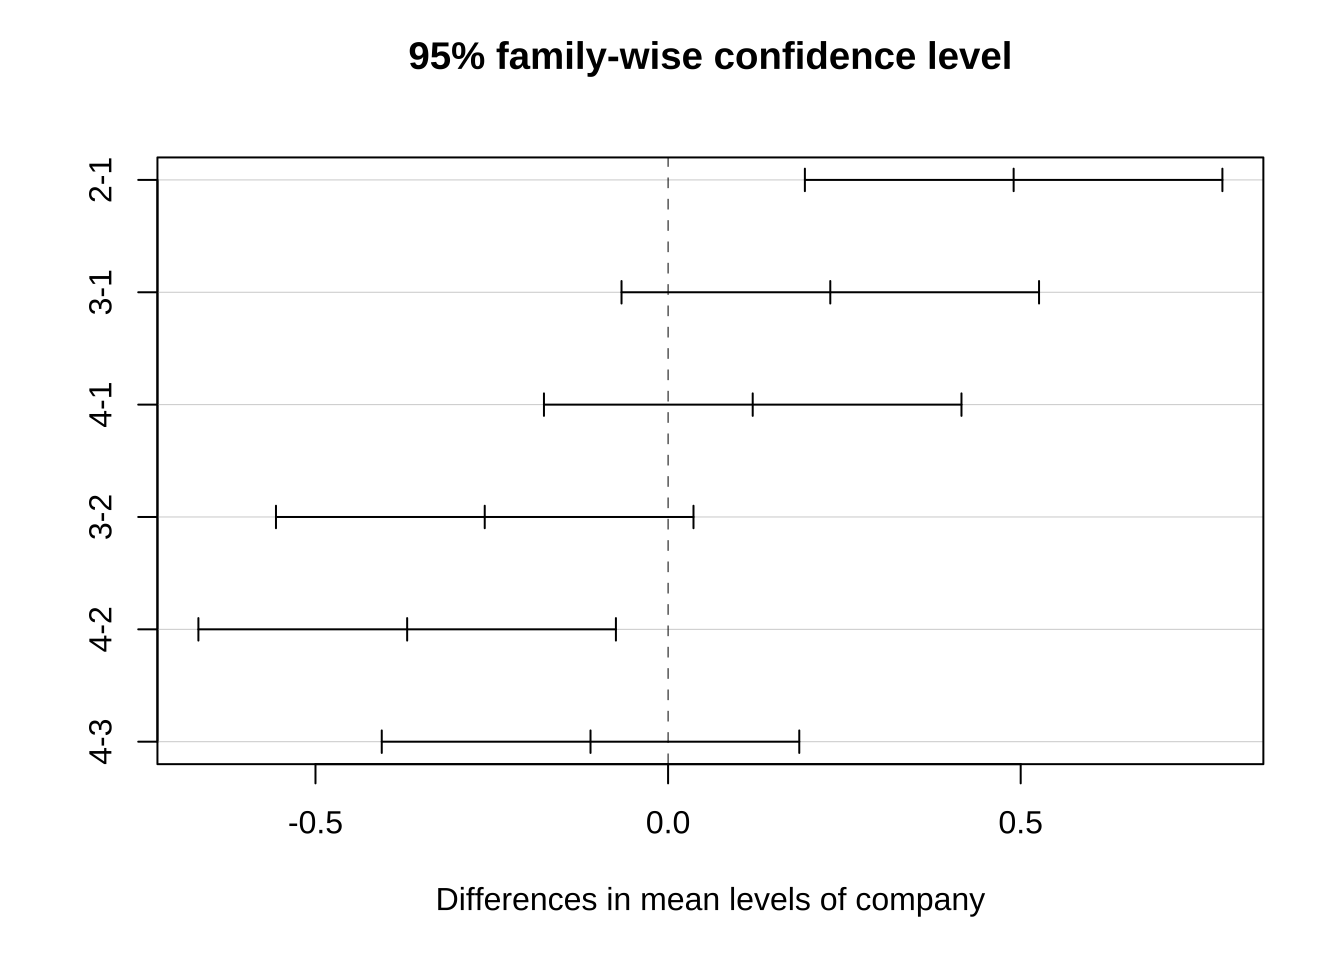
\includegraphics{linearmodel_files/figure-latex/unnamed-chunk-19-1.pdf}

\hypertarget{uxc138-uxbc29uxbc95uxc5d0uxc11cuxc758-p-uxac12-uxbe44uxad50}{%
\subsection{세 방법에서의 p-값 비교}\label{uxc138-uxbc29uxbc95uxc5d0uxc11cuxc758-p-uxac12-uxbe44uxad50}}

위에서 살펴본 수정을 하지 않은 LSD 방법, Tukey의 HSD 방법과 본페로니
방법에서 계산된 p-값을 아래 표에서 비교하였다.

\begin{longtable}[]{@{}rrrr@{}}
\caption{LSD, Bonferoni, HSD 방법의 p-값 비교}\tabularnewline
\toprule
펼균의 비교 조합 & LSD & HSD & Bonf\tabularnewline
\midrule
\endfirsthead
\toprule
펼균의 비교 조합 & LSD & HSD & Bonf\tabularnewline
\midrule
\endhead
1-2 & 0.0004 & 0.0017 & 0.0021\tabularnewline
1-3 & 0.0397 & 0.1509 & 0.2383\tabularnewline
1-4 & 0.2520 & 0.6363 & 1.0000\tabularnewline
2-3 & 0.0229 & 0.0924 & 0.1374\tabularnewline
2-4 & 0.0030 & 0.0137 & 0.0179\tabularnewline
3-4 & 0.2916 & 0.6944 & 1.0000\tabularnewline
\bottomrule
\end{longtable}

  \bibliography{book.bib,packages.bib}

\end{document}
